\documentclass{beamer}

\batchmode

\usepackage{amsmath,amssymb,enumerate,epsfig,bbm,calc,color,ifthen,capt-of}

\usetheme{Berlin}
\usecolortheme{mit}

%% <language_settings> %%
\usepackage[utf8x]{inputenc}
\usepackage[czech]{babel}
%% </language_settings> %%

%% Source code insertions
\usepackage{verbatim}

%% Include images
\usepackage{graphicx}

%% Hyperlinks
\usepackage{hyperref}

%% <change me> %%
\title{Contributing to Gentoo: Getting Involved more}
\author[Markos Chandras \& Tomáš Chvátal]{Markos Chandras $<$hwoarang@gentoo.org$>$ \\ Tomáš Chvátal $<$scarabeus@gentoo.org$>$}
\date{2012/10/21}
%% </change me> %%

%% <logo> %%
\usepackage[absolute,overlay]{textpos}
\setlength{\TPHorizModule}{1mm}
\setlength{\TPVertModule}{1mm}
\newcommand{\MyLogo}{
	\begin{textblock}{14}(110,7)
		\includegraphics[width=14mm,height=14mm]{gentoo-logo.png}
	\end{textblock}
}

\newcommand*\oldmacro{}
\let\oldmacro\insertshorttitle
\renewcommand*\insertshorttitle{
	\MyLogo
	\oldmacro\hfill
}
%% </logo> %%

%% <bgimage> %%
\usebackgroundtemplate{
	
\includegraphics[width=\paperwidth,height=\paperheight]{gentoo-background-1.png}
}
%% </bgimage> %%

%% <ToC Before each section> %%
%\AtBeginSection[]{
%	\begin{frame}<beamer>
%		\frametitle{Přehled}
%		\tableofcontents[currentsection]
%	\end{frame}
%}
%% </ToC Before each section> %%

%% <each bullet on one slide> %%
%% better to use \pause on points where we really want to stop :)
%\beamerdefaultoverlayspecification{<+->}
%% </each bullet on one slide> %%
% -----------------------------------------------------------------------------
\begin{document}
% -----------------------------------------------------------------------------
\frame{\titlepage}
%\section[Přehled]{}
%\begin{frame}{Přehled}
%	\tableofcontents
%\end{frame}
% -----------------------------------------------------------------------------
\section{Introduction}

\subsection{Tomáš}

\begin{frame}{Who is Tomáš Chvátal}
	\begin{itemize}
		\item Council member (currently second term)
		\item KDE team member (former lead)
		\item Libreoffice maintainer
		\item Formely also working on X11, Overlays, Clustering, QA, ...
	\end{itemize}
\end{frame}

\subsection{Markos}
\begin{frame}{And who is Markos Chandras}
Gentoo Developer for 4 years, involved in quite a few areas
\begin{itemize}
	\item Qt
	\item Embedded
	\item Devrel
	\item Recruiter
	\item "Undertaker"
	\item Treecleaner
	\item AMD64
\end{itemize}
Currently working as a Graduate Design Engineer at Imagination Technologies Ltd.
\end{frame}
% -----------------------------------------------------------------------------

% -------------------- here goes hwoarang's presentatons ---------------------
% --------------------- uncomment to include them ----------------------------
% ----------------------- Becoming a Gentoo Developer -------------------------
\section{Recruiting}

\subsection{Becoming a Gentoo Developer}
\begin{frame}{Getting your Gentoo Developer Badge}
Long process, requires time, patience and deep understanding of the Gentoo Organizational and Technical policies.
\\~\\
Required Steps
	\begin{itemize}
		\item Find a mentor!
		\item Ebuild Quiz
		\item End Quiz
		\item Series of interviews with a recruiter
		\item Practical Test
	\end{itemize}
\end{frame}
%------------------------------------------------------------------------------

% ----------------------- What you get as a Developer -------------------------
\begin{frame}{Why?}
Get +w access to our git, svn and gentoo-x86 cvs (a.k.a portage) trees
\\~\\
Also
	\begin{itemize}
		\item \$\{yournickname\}@gentoo.org email (cool huh?)
		\item Improve (or rather serve!) your beloved distro
		\item Experience
		\item Meet new people
		\item Epic flames that you wouldn't want to miss
	\end{itemize}
\end{frame}
%------------------------------------------------------------------------------

%----------------------- Improving Recruitment Process-------------------------
\subsection{Improving the Recruitment Process}
\begin{frame}{What can be done?}
As said, long (like really *really* long) process
\\~\\
Is there room for improvements?
	\begin{itemize}
		\item Improved webapp?
	 	\item Google Docs (either for quiz submission or real-time tests)?
	 	\item G+ Hangouts?
	 	\item Other? Ideas? Please tell me!
	\end{itemize}
\end{frame}
%------------------------------------------------------------------------------

% ----------------------- Recruitment Performance -------------------------
\subsection{How do we perform?}
\begin{frame}{Recruitment Statistics}
	\begin{center}
	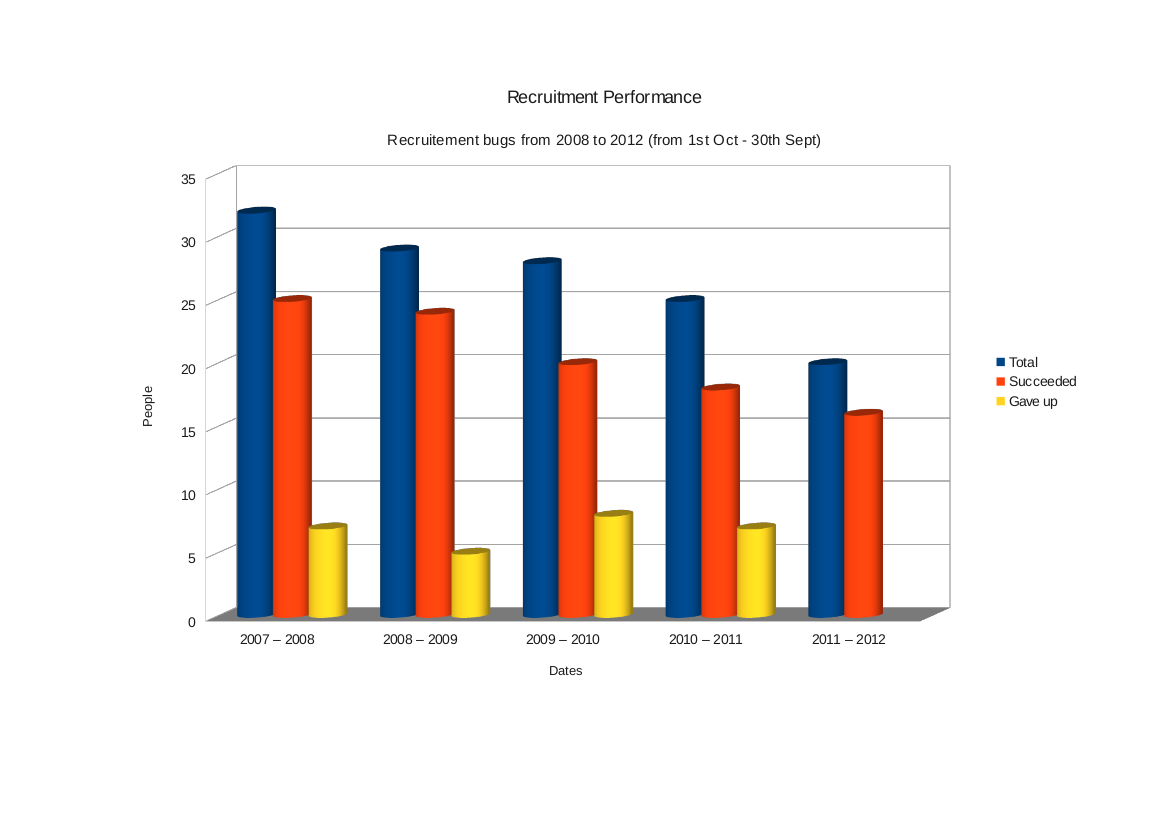
\includegraphics[scale=0.32]{recruitment_stats.png}
	\end{center}
\end{frame}
%------------------------------------------------------------------------------

%------------------------- Proxy Maintainers ----------------------------------
\subsection{Other ways to help us}
\begin{frame}{Proxy Maintainers}
	\begin{center}
	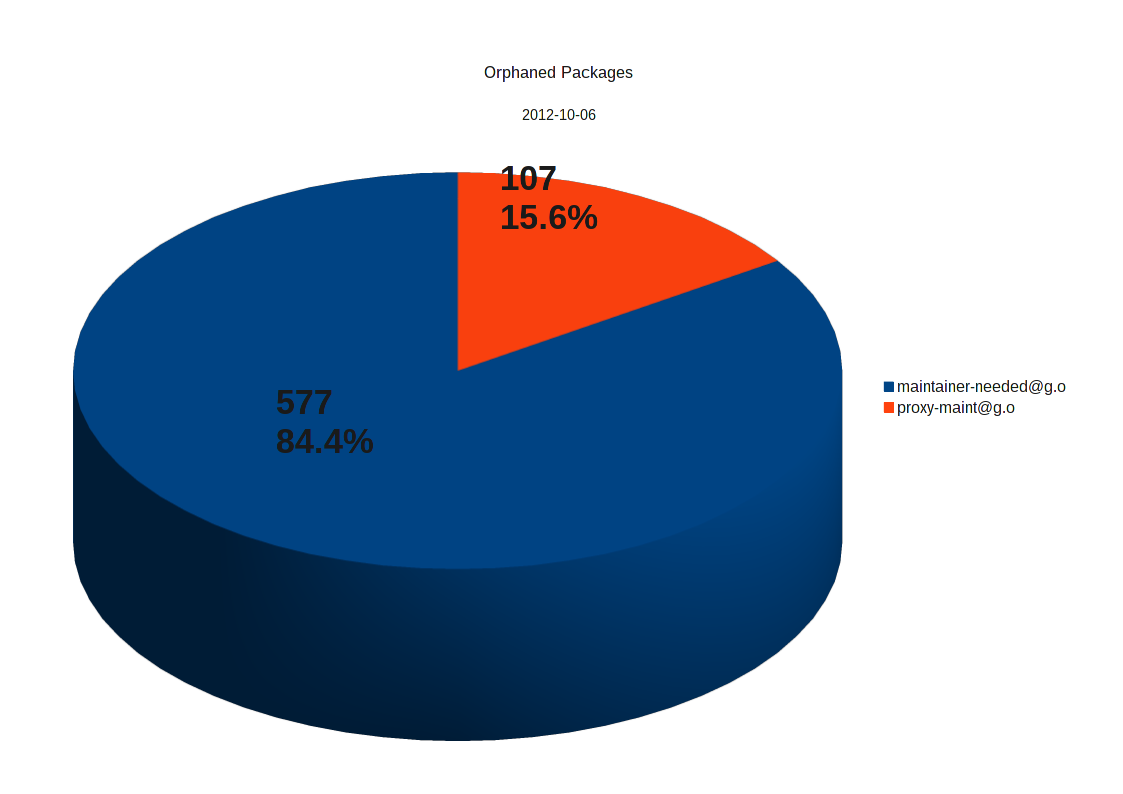
\includegraphics[scale=0.28]{orphaned_packages.png}
	\end{center}
\end{frame}
%------------------------------------------------------------------------------

%------------------------- AT/HT ----------------------------------
\begin{frame}{Arch / Herd Testers}
All we need is your CPU cycles (Ok and some RAM too)
	\begin{itemize}
	\item AT: Use your stable amd64/x86/\$\{arch\} box to help us stabilize more packages
	\item HT: Build, run, crash the testing packages for your favorite herd (kde, lxde, chromium etc.). Less work for ATs ;-)
	\end{itemize}
\end{frame}
%------------------------------------------------------------------------------

%---------------------- Help Needed -------------------------------------------
\subsection{We need help}
\begin{frame}{Where do we need help?}
	\begin{itemize}
		\item \href{http://www.gentoo.org/proj/en/devrel/staffing-needs/}{http://www.gentoo.org/proj/en/devrel/staffing-needs/}
		\item \href{http://www.gentoo.org/proj/en/qa/treecleaners/maintainer-needed.xml}{http://www.gentoo.org/proj/en/qa/treecleaners/maintainer-needed.xml}
		\item Search for long-standing open bugs, submit patches, then contact proxy-maint@gentoo.org
		\item We are always looking for new people even if you don't know what you want to do
	\end{itemize}
\begin{center}Contact us: recruiters@gentoo.org\end{center}
\end{frame}
%------------------------------------------------------------------------------


\section{Contributing code wise}

\subsection{Ebuild example}

\begin{frame}{net-dns/knot}
	\begin{center}net-dns/knot example and explanation.\end{center}
\end{frame}

\subsection{Simple eclass}

\begin{frame}{base.eclass and git-2.eclass}
        \begin{center}Eclass example and explanation.\end{center}
\end{frame}

\subsection{Repoman usage}

\begin{frame}{Why/how to use repoman}
	\begin{itemize}
		\item Always fix all the issues to ease up overall QA. 
		\item The minorsyn warnings can be ignored.
		\item use of -f (--force) should be really avoided unless really required.
	\end{itemize}
\end{frame}


% -----------------------------------------------------------------------------
\section{Wrap-up}

\subsection{Wrap-up}

\begin{frame}{Links to learn from and links to stuff I mentioned}
	\begin{itemize}
		\item http://www.gentoo.org/proj/en/devrel/recruiters/
		\item http://www.gentoo.org/proj/en/qa/
	\end{itemize}
\end{frame}

\begin{frame}{Questions}
	\begin{center}Nobody wants to ask anything. Right?\end{center}
\end{frame}

\begin{frame}{Thank you}
	\begin{center}Thank you for your attention!\end{center}
\end{frame}
% -----------------------------------------------------------------------------
\end{document}
